\documentclass{article}
\usepackage[a4paper,width=150mm,top=25mm,bottom=25mm,bindingoffset=6mm]{geometry}

\usepackage{float}
\usepackage{amsmath}
\usepackage[english]{babel}
\usepackage[utf8x]{inputenc}
\usepackage{graphicx}
\usepackage[colorinlistoftodos]{todonotes}
\usepackage{listings}
\usepackage{color}
\usepackage{multirow}
\newcommand\numberthis{\addtocounter{equation}{1}\tag{\theequation}}

\lstset{
language=R,
basicstyle=\scriptsize\ttfamily,
commentstyle=\ttfamily\color{green},
numbers=left,
numberstyle=\ttfamily\color{blue}\footnotesize,
stepnumber=1,
numbersep=5pt,
backgroundcolor=\color{white},
showspaces=false,
showstringspaces=false,
showtabs=false,
%frame=single,
tabsize=2,
captionpos=b,
breaklines=true,
breakatwhitespace=false,
title=\lstname,
escapeinside={},
keywordstyle={},
morekeywords={}
} 
\usepackage{enumitem}
\usepackage{subcaption}
\usepackage{parskip}

\title{Simulation of Chord Peer-to-peer Network: \\
Distributed System (Graduate Course)}

\author{Chih-Yuan Lin \\
chih-yuan.lin@liu.se \\
Department of Computer and Information Science\\
Linköping University\\}
\begin{document}
\maketitle
\begin{center}
--------------------------------------------------------------------------------\\
\end{center}

\section*{Introduction}
%Write a basic simulator (in the language of your choice) that simulates the Chord peer-to-peer protocol.  
%Your code should support (i) node insertion and (ii) message forwarding.  
%Then, simulate example scenarios and report how the overhead of node insertion and packet forwarding scales with the number of nodes in your Chord implementation.  
%Your report should reflect on your findings and compare with results from the existing literature.
This report summarizes the project work of the Distributed System course. Our assignment was to implement a basic simulator of Chord peer-to-peer network proposed by Stoica et al \cite{paper, report} and measure the overhead of node insertion and message forwarding scales with the number of nodes. The report first introduces the Chord algorithm in the first section and then describes our implementation in the second section. Finally, it shows the settings and results of experiments and compares the results with the proposed performance in the original papers.

\section*{Background}
Chord is a scalable peer-to-peer lookup service for Internet applications. Each Chord node has a unique $m$-bit identifier (ID) locating in a virtual ID cycle. Given a key, Chord defines the node which is responsible for the key to be the successor of the key's ID. The successor of an ID $j$ is the node with the smallest ID that is greater than or equal to $j$. 

A Chord node needs two data structures to perform lookups: a successor list and a finger table. Lookups performed only with successor list would require an average $N/2$ message exchanges, where $N$ is the number of nodes. To reduce the number of message exchanges to average $\frac{1}{2}logN$, each node remains a finger table with $m$ entries. The $i^{th}$ entry in the table at node $n$ contains the ID of the first node that succeeds $n$ by at least $2^{i-1}$ on the circular space. Fig. \ref{alg.lookup} shows pseudo-code to complete a lookup operation. If a key's ID falls between $n$ and its successor, node $n$ returns its successor. Otherwise, node $n$ searches its finger table for the node $n^\prime$ whose ID most closely precedes the key's ID and then ask $n^\prime$ to find the key's successor.

Fig. \ref{alg.insert} shows pseudo-code to node insertion. When a new node $n$ joins the network, Chord must perform
\begin{enumerate}
\item initialize the predecessor and finger table of node $n$ ($init\_finger\_table$).
\item Update the finger tables and predecessors of existing nodes to reflect the insertion of $n$ ($update\_others$).
\end{enumerate}
In function $init\_finger\_table$: Node $n$ checks whether the $i^{th}$ fingers is also the correct $(i+1)^{th}$ finger for each $i$. If not, $n$ learns the finger value by asking $n^\prime$ to look it up. That is, the total number of fingers that must be looked up to $O(logN)$, where induces the overall time to $O(log^2N)$.

In function $update\_others$: For a give $n$, the algorithm finds node $p$ whose $i^{th}$ finger might be $n$ counter-clock-wisely. The number of nodes that need to be updated is proposed as $O(logN)$ with high probability. Finding and updating these nodes takes overall $O(log^2N)$.

\begin{figure}[H]
\centering
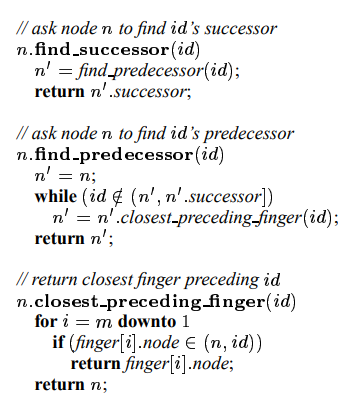
\includegraphics[scale=1.5]{alg_lookup.PNG}
\caption{The proposed lookup algorithm.
\label{alg.lookup}}
\end{figure}


\begin{figure}[H]
\centering
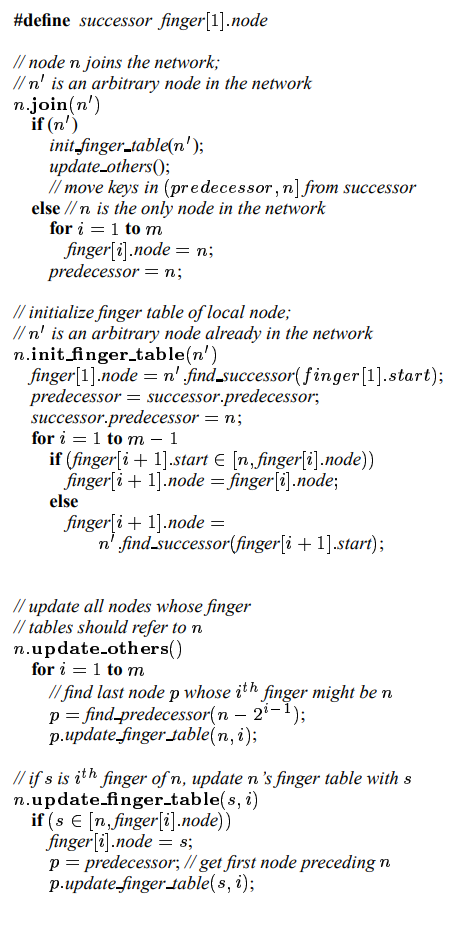
\includegraphics[scale=1.5]{alg_insert.PNG}
\caption{The proposed node insertion algorithm.
\label{alg.insert}}
\end{figure}


\section*{Implementation}
Our simulator was implemented with Python in an object-oriented manner. A Chord network is maintained by a list of Node instances. Messages are forwarded as arguments between public methods of two instances (i.e, without passing through RPC). Fig. \ref{node} shows the class variables and methods. 

In this project, we implement a simple Chord-based lookup service. Each Chord node has a variable \textit{ip} keeping its IP address and an \textit{ID\_LEN}-long \textit{id} which is produced by hashing the IP address with SHA-1 function. To improve the scalability, Chord protocol requires more routing information than just a successor pointer. Variable \textit{predecessor} is the predecessor pointer and \textit{fingers} is the finger table. The finger table contains \textit{ID\_LEN} entries. The $i^{th}$ entry of node $n$ stores the pointer of the first node, $s$, that succeeds $n$ by at least $2^i$, where $1 \leq i \leq m$. Last, we implement the storage with the build-in dictionary data type, that stores pairs of strings and secret numbers.
\begin{figure}[H]
\centering
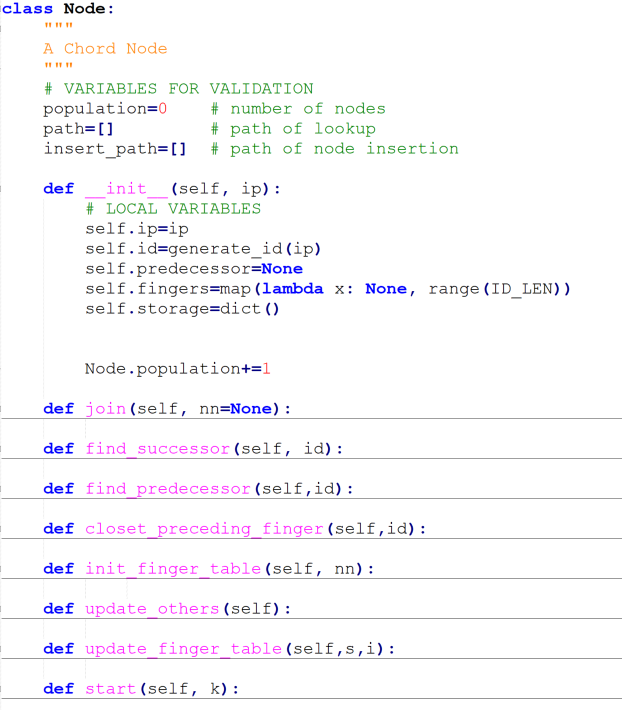
\includegraphics[scale=1.5]{Node.PNG}
\caption{The Node class.
\label{node}}
\end{figure}

We also provide three APIs to manipulate the Chord network as shown in Fig. \ref{api}
\begin{enumerate}
\item Key location
\item Lookup
\item Node insertion
\end{enumerate}
We test only the Lookup and Node insertion as required.
\begin{figure}[H]
\centering
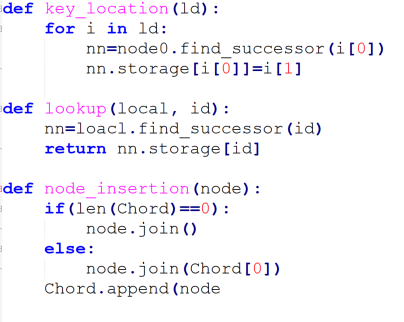
\includegraphics[scale=1.5]{APIs.PNG}
\caption{The defined APIs
\label{api}}
\end{figure}

\section*{Performance}
This section describes how we measure the overhead of node insertion and message forwarding and the resulting performance.
\subsection*{Experiment Settings}
\textbf{Message forwarding.} Message forwarding in a Chord network is triggered by a lookup operation. The original paper evaluates the lookup performance with the metric path length, which is defined as the number of nodes traversed during a lookup operation. The paper presents the path length in a network that contains $2^k$ random nodes and $100 \times 2^k$ random keys in all. It varies the $k$ from $3$ to $14$ and conducts an separate experiment for each $k$. Each node in each experiment picked a random set of keys to query from the system, and it measures the path length required to resolve each query on average. In order to compare our work with the original paper, we follow the same settings of experiments.


\textbf{Node insertion.} Node insertion performance is not tested in the original paper. Thus, we extend the definition of path length here. We measure the number of nodes traversed during \textit{init\_finger\_table} and \textit{update\_finger\_table} and refer to this measurement as path length of node insertion. Our experiments to measure the overhead of node insertion are conducted in the same Chord networks as the above. For each experiment, we insert a random node into a $2^k$ random network. We repeats the experiment $20$ times for each $k$.

\subsection*{Results}
Fig. \ref{lookup} presents the median, $1^{st}$, and $99^{th}$ percentiles of path length of lookup as a function of $k$. The red line is generated by $\frac{1}{2}logN$ as mentioned in the background section. We can see that the path length increases logarithmically as proposed. Compare to the proposed performance in Fig. \ref{oldlookup}, the length of routing path is quite similar. 
\begin{figure}[H]
\centering
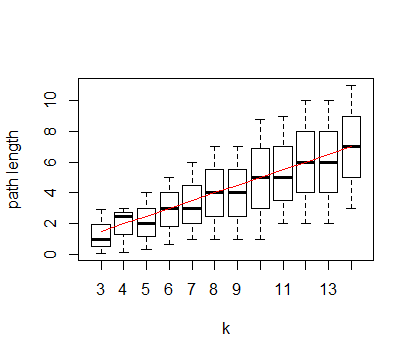
\includegraphics[scale=1]{lookup.png}
\caption{The path length of lookup operation as a function of $k$.
\label{lookup}}
\end{figure}

\begin{figure}[H]
\centering
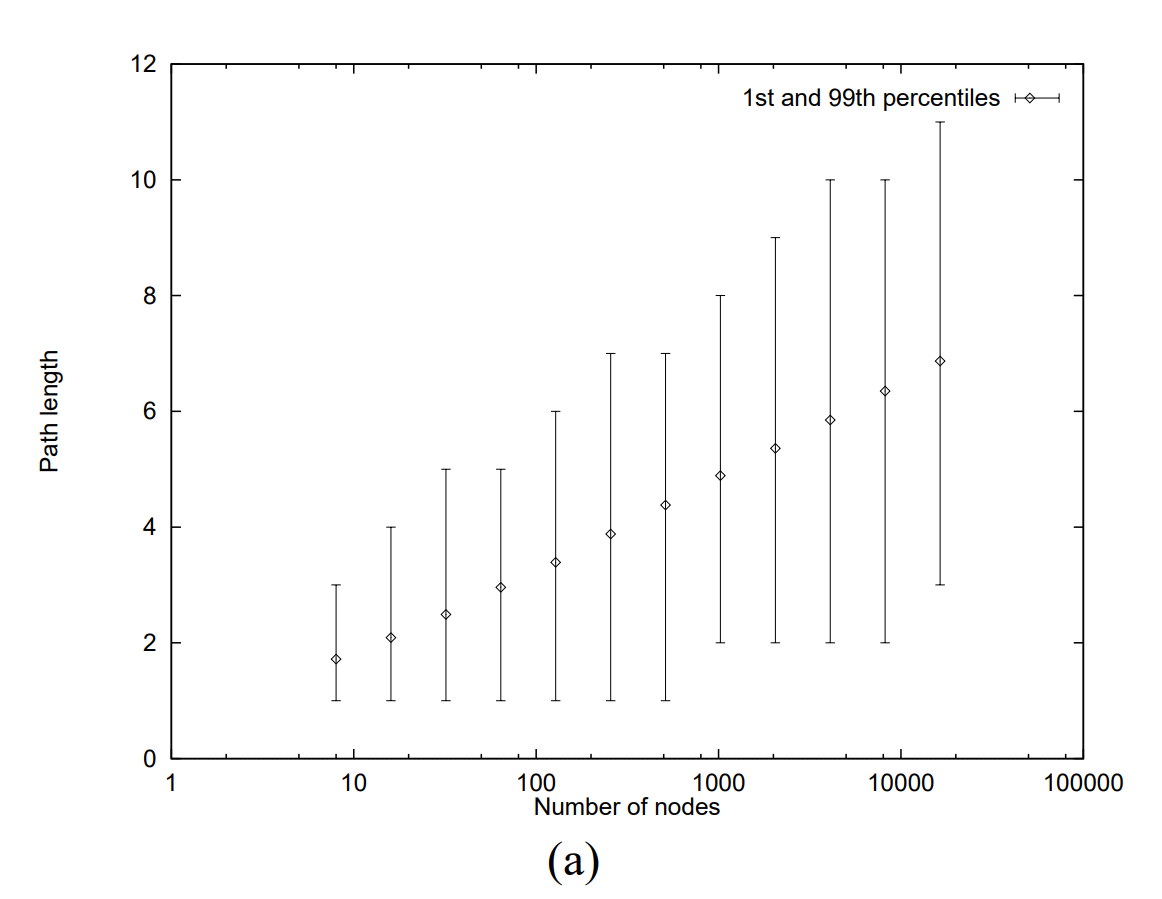
\includegraphics[scale=1]{oldlookup.PNG}
\caption{The path length of lookup operation as a function of network size.
\label{oldlookup}}
\end{figure}

Fig.\ref{insert} shows the median, $1^{st}$, and $99^{th}$ percentiles of path length of node insertion as a function of $k$. The red line is generated by $200+4.5log^2N$, where the coefficients are determined experimentally. The concludes the performance of insertion is $O(log^2N)$ as mentioned in the background section. 
\begin{figure}[H]
\centering
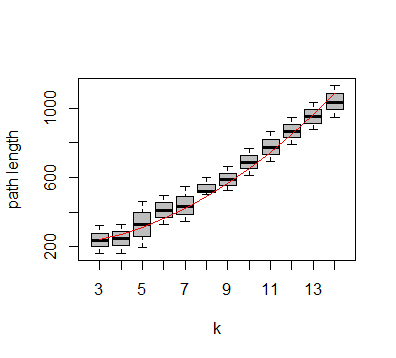
\includegraphics[scale=1]{insertion.png}
\caption{The path length of node insertion as a function of $k$
\label{insert}}
\end{figure}


%\begin{equation}
%K(u)=exp(-\parallel u \parallel^2).
%\end{equation}



\bibliographystyle{unsrt}
\bibliography{refs}

\end{document}



